\section{类SampledSpectrum}\label{sec:类SampledSpectrum}
\refvar{SampledSpectrum}{}用\refvar{CoefficientSpectrum}{}基础结构
来表示在起始和结束波长之间均匀间隔采样的SPD。
波长覆盖范围从400nm到700nm——人类视觉系统最为敏感的可见光谱范围。
样本数量60一般足够为渲染准确表示复杂的SPD
(见“扩展阅读”一节了解SPD采样率要求的背景)。
因此,第一个样本表示波长范围$[400,405)$,第二个表示$[405,410)$,以此类推。
这些值很容易在此处按需修改。
\begin{lstlisting}
`\initcode{Spectrum Utility Declarations}{=}\initnext{SpectrumUtilityDeclarations}`
static const int `\initvar{sampledLambdaStart}{}` = 400;
static const int `\initvar{sampledLambdaEnd}{}` = 700;
static const int `\initvar{nSpectralSamples}{}` = 60;
\end{lstlisting}
\begin{lstlisting}
`\refcode{Spectrum Declarations}{+=}\lastnext{SpectrumDeclarations}`
class `\initvar{SampledSpectrum}{}` : public `\refvar{CoefficientSpectrum}{}`<`\refvar{nSpectralSamples}{}`> {
public:
    `\refcode{SampledSpectrum Public Methods}{}`
private:
    `\refcode{SampledSpectrum Private Data}{}`
};
\end{lstlisting}

通过从类\refvar{CoefficientSpectrum}{}继承,
\refvar{SampledSpectrum}{}自动拥有之前定义的所有基本光谱算术运算符。
留待为它定义的主要方法是从光谱数据初始化它以及将它表示的SPD转换为其他光谱表示(例如RGB)。
用常数SPD初始化它的构造函数很简单。
\begin{lstlisting}
`\initcode{SampledSpectrum Public Methods}{=}\initnext{SampledSpectrumPublicMethods}`
`\refvar{SampledSpectrum}{}`(`\refvar{Float}{}` v = 0.f) : `\refvar{CoefficientSpectrum}{}`(v) { }
\end{lstlisting}

光谱数据经常以一组样本$(\lambda_i,v_i)$提供给我们,
其中第$i$个样本有在波长$\lambda_i$处的某值$v_i$。
一般而言,样本可能有不规则间隔,可能比\refvar{SampledSpectrum}{}要存储的更多或更少
(见pbrt发行中路径{\ttfamily scenes/spds}下\sidenote{译者注:笔者没有找到该路径。}
pbrt所用的各种SPD,它们许多都有不规则间隔)。

方法\refvar[SampledSpectrum::FromSampled]{FromSampled}{()}取用在
给定波长{\ttfamily lambda}处的SPD样本值{\ttfamily v}数组
并用它们定义分段线性函数来表示SPD。
对于\refvar{SampledSpectrum}{}的每个SPD样本,
它用下面定义的功能函数\refvar{AverageSpectrumSamples}{()}
来计算分段线性函数在每个SPD样本对应的波长范围上的均值。
\begin{lstlisting}
`\refcode{SampledSpectrum Public Methods}{+=}\lastnext{SampledSpectrumPublicMethods}`
static `\refvar{SampledSpectrum}{}` `\initvar[SampledSpectrum::FromSampled]{FromSampled}{}`(const `\refvar{Float}{}` *lambda,
                                   const `\refvar{Float}{}` *v, int n) {
    `\refcode{Sort samples if unordered, use sorted for returned spectrum}{}`
    `\refvar{SampledSpectrum}{}` r;
    for (int i = 0; i < `\refvar{nSpectralSamples}{}`; ++i) {
        `\refcode{Compute average value of given SPD over th sample's range}{}`
    }
    return r;
}
\end{lstlisting}

函数\refvar{AverageSpectrumSamples}{()}要求值$(\lambda_i,v_i)$按波长排序。
{\initvar{SpectrumSamplesSorted}{()}}函数检查它们是不是;
如果不是,则{\initvar{SortSpectrumSamples}{()}}对它们排序。
注意我们为排序的样本分配新存储而不改变调用者传入的值;
一般而言,对于该函数(不需要担心其特定实现的这些要求)的用户
这样做可能并不是期望的行为。
我们这里不会介绍这两个函数的实现,因为它们很简单。
\begin{lstlisting}
`\initcode{Sort samples if unordered, use sorted for returned spectrum}{=}`
if (!`\refvar{SpectrumSamplesSorted}{}`(lambda, v, n)) {
    std::vector<`\refvar{Float}{}`> slambda(&lambda[0], &lambda[n]);
    std::vector<`\refvar{Float}{}`> sv(&v[0], &v[n]);
    `\refvar{SortSpectrumSamples}{}`(&slambda[0], &sv[0], n);
    return `\refvar[SampledSpectrum::FromSampled]{FromSampled}{}`(&slambda[0], &sv[0], n);
}
\end{lstlisting}

为计算第$i$个光谱样本的值,我们计算其对应的波长范围——
{\ttfamily lambda0}到{\ttfamily lambda1}——
并用函数\refvar{AverageSpectrumSamples}{()}计算该范围给定分段线性SPD的均值。
这是采样和重构的1D实例,第\refchap{采样与重构}会讨论该话题的更多细节。
\begin{lstlisting}
`\initcode{Compute average value of given SPD over th sample's range}{=}`
`\refvar{Float}{}` lambda0 = `\refvar{Lerp}{}`(`\refvar{Float}{}`(i) / `\refvar{Float}{}`(`\refvar{nSpectralSamples}{}`), 
                     `\refvar{sampledLambdaStart}{}`, `\refvar{sampledLambdaEnd}{}`);
`\refvar{Float}{}` lambda1 = `\refvar{Lerp}{}`(`\refvar{Float}{}`(i + 1) / `\refvar{Float}{}`(`\refvar{nSpectralSamples}{}`), 
                     `\refvar{sampledLambdaStart}{}`, `\refvar{sampledLambdaEnd}{}`);
r.`\refvar[CoefficientSpectrum::c]{c}{}`[i] = `\refvar{AverageSpectrumSamples}{}`(lambda, v, n, lambda0, lambda1);
\end{lstlisting}

\reffig{5.2}展示了\refvar{AverageSpectrumSamples}{()}采用的基础方法:
它在部分或完全位于波长范围内的样本间的每个线性段上迭代,
从{\ttfamily lambdaStart}到{\ttfamily lambdaEnd}。
对于每个这样的分段,它计算其范围上的均值,
用该段覆盖的波长范围缩放该均值,最后求这些值的和。
最终均值是该和除以整个波长范围。
\begin{figure}[htbp]
    \centering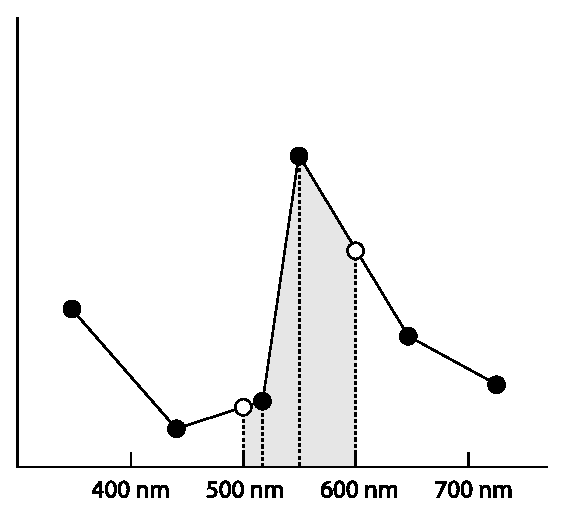
\includegraphics[width=0.4\linewidth]{chap05/IrregularSPDresample.eps}
    \caption{当重采样不规则定义的SPD时,我们需要计算由SPD样本定义的
        分段线性函数的均值。这里,我们想求从500nm到600nm的均值——图像下的阴影区。
        函数\refvar{AverageSpectrumSamples}{()}通过计算该图中虚线表示的每个区域的面积来完成。}
    \label{fig:5.2}
\end{figure}

\begin{lstlisting}
`\initcode{Spectrum Method Definitions}{=}\initnext{SpectrumMethodDefinitions}`
`\refvar{Float}{}` `\initvar{AverageSpectrumSamples}{}`(const `\refvar{Float}{}` *lambda, const `\refvar{Float}{}` *vals,
        int n, `\refvar{Float}{}` lambdaStart, `\refvar{Float}{}` lambdaEnd) {
    `\refcode{Handle cases with out-of-bounds range or single sample only}{}`
    `\refvar{Float}{}` sum = 0;
    `\refcode{Add contributions of constant segments before/after samples}{}`
    `\refcode{Advance to first relevant wavelength segment}{}`
    `\refcode{Loop over wavelength sample segments and add contributions}{}`
    return sum / (lambdaEnd - lambdaStart);
}
\end{lstlisting}

该函数从检查和处理极端情况开始,即求均值的波长范围
超出了提供的波长范围或只有单个样本进而均值计算是平凡的情况。
我们假设SPD在超出提供的采样范围外有常值(在两个端点的值);
如果这对于特定数据集不是一个合理的假设,则提供的数据应该在端点处有显式值(例如)0。
\begin{lstlisting}
`\initcode{Handle cases with out-of-bounds range or single sample only}{=}`
if (lambdaEnd   <= lambda[0])     return vals[0];
if (lambdaStart >= lambda[n - 1]) return vals[n - 1];
if (n == 1) return vals[0];
\end{lstlisting}

处理了这些情况后,下一步是检查看求均值的范围是否有部分超出第一个和/或最后一个样本值。
如果是,则我们累积常数段的贡献,用超出边界的波长范围缩放它。
\begin{lstlisting}
`\initcode{Add contributions of constant segments before/after samples}{=}`
if (lambdaStart < lambda[0])
    sum += vals[0] * (lambda[0] - lambdaStart);
if (lambdaEnd > lambda[n-1])
    sum += vals[n - 1] * (lambdaEnd - lambda[n - 1]);
\end{lstlisting}

现在我们推进到首个索引{\ttfamily i},
插值范围的起始波长重合于从$\lambda_i$到$\lambda_{i+1}$的一段。
这里更高效的实现是用二叉搜索而不是线性搜索
\footnote{甚至更高效的实现是利用一个事实即调用代码一般会需要
    在一段相邻波长范围上插值后的值,并可能在单次调用中接收了全部范围。
    然后可以为下一次插值从上一结尾处开始逐步寻找起始索引。}。
然而,该代码目前只在场景初始化时调用,所以目前不优化它不会影响渲染性能。
\begin{lstlisting}
`\initcode{Advance to first relevant wavelength segment}{=}`
int i = 0;
while (lambdaStart > lambda[i + 1]) ++i;
\end{lstlisting}

下面的循环在与求均值的范围重合的每个线性段上迭代。
对于每一段,它都通过求函数在这两点上取值的均值来
计算在波长范围{\ttfamily segLambdaStart}到{\ttfamily segLambdaEnd}上的均值。
该值依次用{\ttfamily interp()}计算,它是在给定波长的两个端点间线性插值的匿名函数。

下面调用{\ttfamily std::min()}和{\ttfamily std::max()}计算波长范围以在该段内做平均;
注意它们自然处理了{\ttfamily lambdaStart}、{\ttfamily lambdaEnd}或两者都在当前段内的情况。
\begin{lstlisting}
`\initcode{Loop over wavelength sample segments and add contributions}{=}`
auto interp = [lambda, vals](`\refvar{Float}{}` w, int i) {
    return `\refvar{Lerp}{}`((w - lambda[i]) / (lambda[i + 1] - lambda[i]),
                vals[i], vals[i + 1]);
};
for (; i+1 < n && lambdaEnd >= lambda[i]; ++i) {
    `\refvar{Float}{}` segLambdaStart = std::max(lambdaStart, lambda[i]);
    `\refvar{Float}{}` segLambdaEnd =   std::min(lambdaEnd,   lambda[i + 1]);
    sum += 0.5 * (interp(segLambdaStart, i) + interp(segLambdaEnd, i)) *
        (segLambdaEnd - segLambdaStart);
}
\end{lstlisting}

\subsection{XYZ颜色}\label{sub:XYZ颜色}
人类视觉系统的一个非凡性质是可只用三个浮点数为人类感知表示颜色。
颜色感知的\keyindex{三刺激理论}{tristimulus theory}{}说
用三个值$x_{\lambda},y_{\lambda}$和$z_{\lambda}$就能为人类观察者准确表示所有可见SPD。
给定发射SPD即$S(\lambda)$,通过积分它们与\keyindex{光谱匹配曲线}{spectral matching curve}{}
$X(\lambda),Y(\lambda)$和$Z(\lambda)$的积可算得这些值:
\begin{align}\label{eq:5.1}
    x_{\lambda} & =\int\limits_{\lambda}{S(\lambda)X(\lambda)\mathrm{d}\lambda}\, ,\nonumber \\
    y_{\lambda} & =\int\limits_{\lambda}{S(\lambda)Y(\lambda)\mathrm{d}\lambda}\, ,          \\
    z_{\lambda} & =\int\limits_{\lambda}{S(\lambda)Z(\lambda)\mathrm{d}\lambda}\, .\nonumber
\end{align}

这些曲线是由国际照明委员会\sidenote{译者注:法文Commission Internationale de l'Éclairage,
    英文International Commission on Illumination,是有关光学、照明、颜色和色度空间科学领域的国际组织,成立于1913年。}(CIE)
规范化机构在一系列以人类为测试对象的实验后决定的并画于\reffig{5.3}中。
一般认为这些匹配曲线通常类似于人类视网膜中三种色敏视锥细胞\sidenote{译者注:原文 color-sensitive cone。}的响应。
惊人的是,有截然不同分布的SPD可能有非常接近的$x_{\lambda},y_{\lambda}$和$z_{\lambda}$值。
对于人类观察者,这样的SPD实际上有一样的视觉呈现。
这样的光谱对称为\keyindex{同色异谱}{metamer}{}。
\begin{figure}[htbp]
    \centering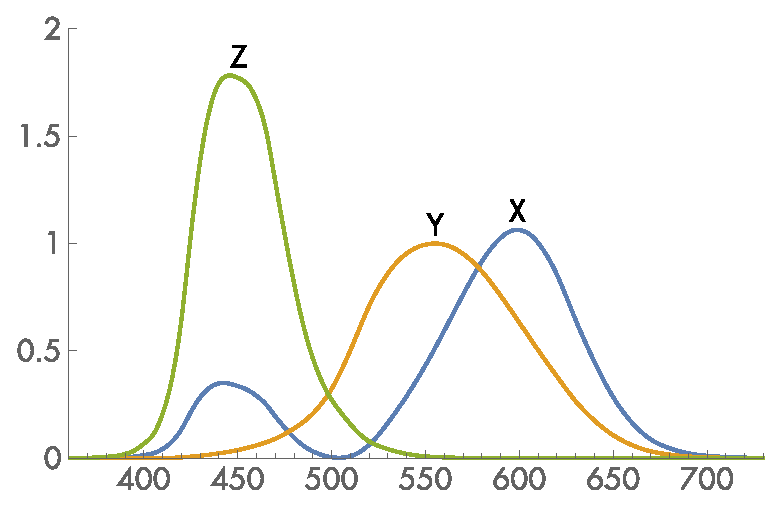
\includegraphics[width=0.5\linewidth]{chap05/matching-xyz.eps}
    \caption{对任意SPD计算XYZ值。用\refeq{5.1}让SPD与三个匹配曲线的每一个
    相乘并在其非零范围上积分以计算$x_{\lambda},y_{\lambda}$和$z_{\lambda}$值。}
    \label{fig:5.3}
\end{figure}

这给我们带来了关于光谱功率分布表示的一个微妙之处。
大部分颜色空间都希望模型颜色是对人类可见的,进而根据颜色感知的三刺激理论只需用三个系数。
尽管XYZ能很好地表示要对人类观察者显示的给定SPD,
但它对于光谱计算而言{\itshape 不是}特别好的基函数集。
例如,尽管XYZ值能很好地分别描述柠檬皮或荧光灯的感知颜色(回想\reffig{5.1}),
但它们各自的XYZ值之积给出的XYZ颜色可能明显不同于用其SPD更精确的表示相乘再计算出的XYZ值。

pbrt提供了标准$X(\lambda),Y(\lambda)$和$Z(\lambda)$相应曲线从360nm到830nm间隔1nm采样的值。
下面的数组中第$i$个样本的波长由\refvar{CIE\_lambda}{}的第$i$个元素给定;
用这种方式显式表示样本波长能更容易将XYZ样本传入到像\refvar{AverageSpectrumSamples}{()}
那样接收波长数组作为参数的函数。
\begin{lstlisting}
`\initcode{Spectral Data Declarations}{=}\initnext{SpectralDataDeclarations}`
static const int `\initvar{nCIESamples}{}` = 471;
extern const `\refvar{Float}{}` `\initvar{CIE\_X}{}`[`\refvar{nCIESamples}{}`];
extern const `\refvar{Float}{}` `\initvar{CIE\_Y}{}`[`\refvar{nCIESamples}{}`];
extern const `\refvar{Float}{}` `\initvar{CIE\_Z}{}`[`\refvar{nCIESamples}{}`];
extern const `\refvar{Float}{}` `\initvar{CIE\_lambda}{}`[`\refvar{nCIESamples}{}`];
\end{lstlisting}

\refvar{SampledSpectrum}{}用这些样本计算其光谱表示里的XYZ匹配曲线(即它们自己是\refvar{SampledSpectrum}{})。
\begin{lstlisting}
`\initcode{SampledSpectrum Private Data}{=}\initnext{SampledSpectrumPrivateData}`
static `\refvar{SampledSpectrum}{}` `\initvar[SampledSpectrum::X]{X}{}`, `\initvar[SampledSpectrum::Y]{Y}{}`, `\initvar[SampledSpectrum::Z]{Z}{}`;
\end{lstlisting}

\refvar{SampledSpectrum}{}的XYZ曲线在方法\refvar{SampledSpectrum::Init}{()}中算得,
它在系统启动时被定义于\refsec{初始化和渲染选项}\sidenote{译者注:原文标错了章节,已修正。}
的函数\refvar{pbrtInit}{()}调用。
\begin{lstlisting}
`\refcode{SampledSpectrum Public Methods}{+=}\lastnext{SampledSpectrumPublicMethods}`
static void `\initvar[SampledSpectrum::Init]{Init}{}`() {
    `\refcode{Compute XYZ matching functions for SampledSpectrum}{}`
    `\refcode{Compute RGB to spectrum functions for SampledSpectrum}{}`
}
\end{lstlisting}
\begin{lstlisting}
`\initcode{General pbrt Initialization}{=}`
`\refvar{SampledSpectrum}{}`::`\refvar[SampledSpectrum::Init]{Init}{}`();
\end{lstlisting}

为\refvar{SampledSpectrum}{}给定波长范围和样本数量,
为每个样本计算匹配函数的值只需计算样本的波长范围并利用\refvar{AverageSpectrumSamples}{()}例程。
\begin{lstlisting}
`\initcode{Compute XYZ matching functions for SampledSpectrum}{=}`
for (int i = 0; i < `\refvar{nSpectralSamples}{}`; ++i) {
    `\refvar{Float}{}` wl0 = `\refvar{Lerp}{}`(`\refvar{Float}{}`(i) / `\refvar{Float}{}`(`\refvar{nSpectralSamples}{}`), 
                     `\refvar{sampledLambdaStart}{}`, `\refvar{sampledLambdaEnd}{}`);
    `\refvar{Float}{}` wl1 = `\refvar{Lerp}{}`(`\refvar{Float}{}`(i + 1) / `\refvar{Float}{}`(`\refvar{nSpectralSamples}{}`), 
                     `\refvar{sampledLambdaStart}{}`, `\refvar{sampledLambdaEnd}{}`);
    `\refvar[SampledSpectrum::X]{X}{}`.`\refvar[CoefficientSpectrum::c]{c}{}`[i] = `\refvar{AverageSpectrumSamples}{}`(`\refvar{CIE\_lambda}{}`, `\refvar{CIE\_X}{}`, `\refvar{nCIESamples}{}`,
                                    wl0, wl1);
    `\refvar[SampledSpectrum::Y]{Y}{}`.`\refvar[CoefficientSpectrum::c]{c}{}`[i] = `\refvar{AverageSpectrumSamples}{}`(`\refvar{CIE\_lambda}{}`, `\refvar{CIE\_Y}{}`, `\refvar{nCIESamples}{}`,
                                    wl0, wl1);
    `\refvar[SampledSpectrum::Z]{Z}{}`.`\refvar[CoefficientSpectrum::c]{c}{}`[i] = `\refvar{AverageSpectrumSamples}{}`(`\refvar{CIE\_lambda}{}`, `\refvar{CIE\_Z}{}`, `\refvar{nCIESamples}{}`,
                                    wl0, wl1);
}
\end{lstlisting}

pbrt中所有\refvar{Spectrum}{}实现都必须提供将其SPD转换为$(x_{\lambda},y_{\lambda},z_{\lambda})$系数的方法。
例如,在更新图像像素的过程中就会调用该方法。
当\refvar{Spectrum}{}表示的沿相机射出的光线上的光提供给\refvar{Film}{}时,
\refvar{Film}{}最终将它们转换为用于存储和/或显示的RGB值时处理的第一步就是将SPD转换为XYZ系数。

为了计算XYZ系数,\refvar{SampledSpectrum}{}用黎曼和计算\refeq{5.1}的积分:
\begin{align*}
    x_{\lambda}\approx\frac{\lambda_{\text{end}}-\lambda_{\text{start}}}{N}\sum\limits_{i=0}^{N-1}{X_ic_i}\, ,
\end{align*}
并以此类推\sidenote{译者注:但是下面的代码中实际上还多除以了{\ttfamily CIE\_Y\_integral}。}。
\begin{lstlisting}
`\refcode{SampledSpectrum Public Methods}{+=}\lastnext{SampledSpectrumPublicMethods}`
void `\initvar{ToXYZ}{}`(`\refvar{Float}{}` xyz[3]) const {
    xyz[0] = xyz[1] = xyz[2] = 0.f;
    for (int i = 0; i < `\refvar{nSpectralSamples}{}`; ++i) {
        xyz[0] += `\refvar[SampledSpectrum::X]{X}{}`.`\refvar[CoefficientSpectrum::c]{c}{}`[i] * `\refvar[CoefficientSpectrum::c]{c}{}`[i];
        xyz[1] += `\refvar[SampledSpectrum::Y]{Y}{}`.`\refvar[CoefficientSpectrum::c]{c}{}`[i] * `\refvar[CoefficientSpectrum::c]{c}{}`[i];
        xyz[2] += `\refvar[SampledSpectrum::Z]{Z}{}`.`\refvar[CoefficientSpectrum::c]{c}{}`[i] * `\refvar[CoefficientSpectrum::c]{c}{}`[i];
    }
    `\refvar{Float}{}` scale = `\refvar{Float}{}`(`\refvar{sampledLambdaEnd}{}` - `\refvar{sampledLambdaStart}{}`) /
                  `\refvar{Float}{}`(CIE_Y_integral * `\refvar{nSpectralSamples}{}`);
    xyz[0] *= scale;
    xyz[1] *= scale;
    xyz[2] *= scale;
}
\end{lstlisting}

XYZ颜色的$y$系数与\keyindex{光亮度}{luminance}{}密切相关,
它度量颜色的感知亮度\sidenote{译者注:原文brightness。}。
亮度将在\refsub{光亮度与光度学}详细介绍。
我们提供了分开的方法单独计算$y$,因为经常只需要光谱的亮度
(例如第\refchap{光传输I:表面反射}、\refchap{光传输II:体积渲染}和\refchap{光传输III:双向方法}中的
一些光传输算法用亮度作为穿过场景的光路的相对重要性度量)。
\begin{lstlisting}
`\refcode{SampledSpectrum Public Methods}{+=}\lastnext{SampledSpectrumPublicMethods}`
`\refvar{Float}{}` `\initvar[SampledSpectrum::y]{y}{}`() const { 
    `\refvar{Float}{}` yy = 0.f;
    for (int i = 0; i < `\refvar{nSpectralSamples}{}`; ++i)
        yy += `\refvar[SampledSpectrum::Y]{Y}{}`.`\refvar[CoefficientSpectrum::c]{c}{}`[i] * `\refvar[CoefficientSpectrum::c]{c}{}`[i];
    return yy * `\refvar{Float}{}`(`\refvar{sampledLambdaEnd}{}` - `\refvar{sampledLambdaStart}{}`) /
        `\refvar{Float}{}`(`\refvar{nSpectralSamples}{}`);
}
\end{lstlisting}

\subsection{RGB颜色}\label{sub:RGB颜色}

当我们在显示器上显示RGB颜色时,实际展示的光谱基本上决定于三种光谱响应曲线的加权和,
红、绿、蓝各一种,由显示器的磷光体\sidenote{译者注:原文phosphor。}发出,例如LED
\sidenote{译者注:即light-emitting diode,发光二极管。}
或LCD\sidenote{译者注:即liquid-crystal display,液晶显示器。}元素,
或者等离子体胞\sidenote{译者注:原文plasma cell。}
\footnote{该模型确实作了简化,它忽略了显示器所作的任何额外处理;
    尤其是许多显示器对显示的值执行了非线性重映射。}。
\reffig{5.4}画出了LED显示器和LCD显示器发出的红、绿和蓝分布;
注意它们截然不同。
\begin{figure}[htbp]
    \centering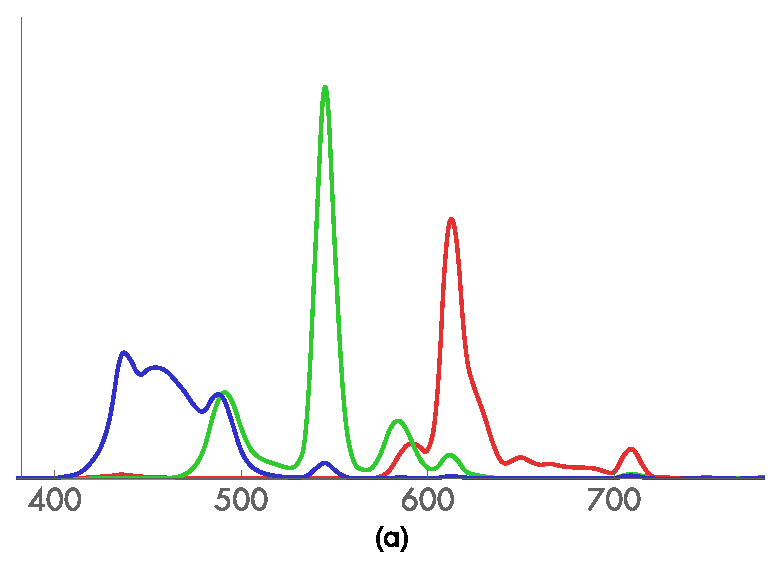
\includegraphics[width=0.45\linewidth]{chap05/lcd-display-spd.eps}\,
    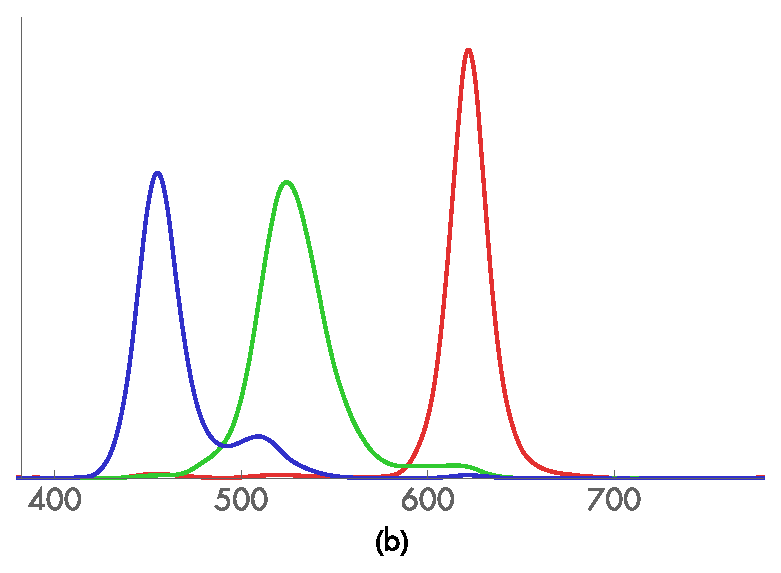
\includegraphics[width=0.45\linewidth]{chap05/led-display-spd.eps}
    \caption{LCD显示器和LED显示器的红、绿和蓝发射曲线。
    第一幅图展示了LCD显示器的曲线,第二幅图展示了LED的。
    这两种显示器有完全不同的发射配置({\itshape 感谢X-Rite公司提供数据})。}
    \label{fig:5.4}
\end{figure}

\reffig{5.5}依次展示了在这些显示器上显示RGB颜色$(0.6,0.3,0.2)$的SPD结果。
不出意料,结果中SPD也截然不同。这个例子说明了当用户选择RGB值时,
用他们提供的RGB值来描述特定颜色实际上只有在给定他们所用的显示器特性知识时才有意义。
\begin{figure}[htbp]
    \centering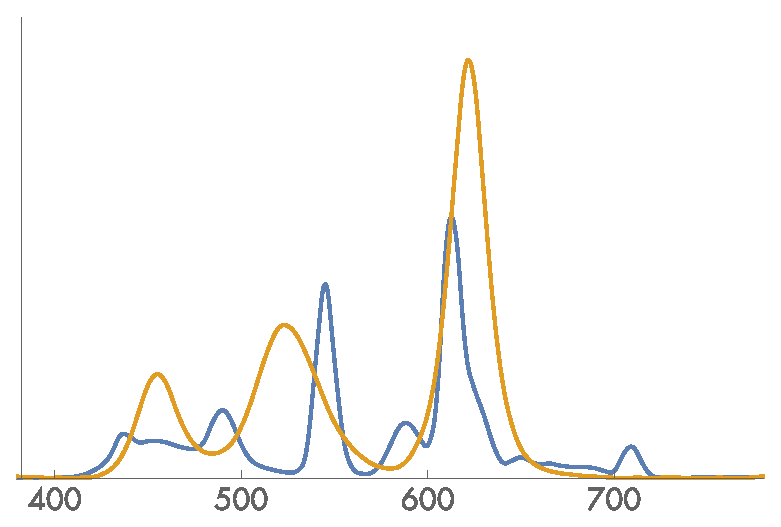
\includegraphics[width=0.5\linewidth]{chap05/same-rgb-different-display.eps}
    \caption{在LED和LCD显示器上显示RGB颜色$(0.6,0.3,0.2)$的SPD。
        甚至给定相同RGB值时得到的发射SPD也明显不同,因为\reffig{5.4}中的发射曲线不同。}
    \label{fig:5.5}
\end{figure}

给定SPD的表示$(x_{\lambda},y_{\lambda},z_{\lambda})$,
为感兴趣的显示器选定好定义红、绿和蓝的特定SPD集后,
我们可以将其转换为相应的RGB系数。
对于特定显示器,有了光谱响应曲线$R(\lambda),G(\lambda)$和$B(\lambda)$后,
可以通过积分响应曲线和SPD即$S(\lambda)$以及利用颜色感知的三刺激理论算得RGB系数:
\begin{align*}
    r & =\int R(\lambda)S(\lambda)\mathrm{d}\lambda=\int R(\lambda)(x_{\lambda}X(\lambda)+y_{\lambda}Y(\lambda)+z_{\lambda}Z(\lambda))\mathrm{d}\lambda                        \\
      & =x_{\lambda}\int R(\lambda)X(\lambda)\mathrm{d}\lambda+y_{\lambda}\int R(\lambda)Y(\lambda)\mathrm{d}\lambda+z_{\lambda}\int R(\lambda)Z(\lambda)\mathrm{d}\lambda\, .
\end{align*}

对于给定的响应曲线可以预先计算积$R(\lambda)X(\lambda)$的积分等,
使得能够把整个转换表达为矩阵:
\begin{align*}
    \left[\begin{array}{c}
            r \\ g\\ b
        \end{array}\right]=\left[
        \begin{array}{ccc}
            \int R(\lambda)X(\lambda)\mathrm{d}\lambda & \int R(\lambda)Y(\lambda)\mathrm{d}\lambda & \int R(\lambda)Z(\lambda)\mathrm{d}\lambda \\
            \int G(\lambda)X(\lambda)\mathrm{d}\lambda & \int G(\lambda)Y(\lambda)\mathrm{d}\lambda & \int G(\lambda)Z(\lambda)\mathrm{d}\lambda \\
            \int B(\lambda)X(\lambda)\mathrm{d}\lambda & \int B(\lambda)Y(\lambda)\mathrm{d}\lambda & \int B(\lambda)Z(\lambda)\mathrm{d}\lambda
        \end{array}
        \right]\left[\begin{array}{c}
            x_{\lambda} \\ y_{\lambda} \\ z_{\lambda}
        \end{array}\right]\, .
\end{align*}

pbrt中实现的转换例程是基于为高清电视定义的RGB光谱标准集的
\sidenote{译者注:这些系数的来由可见译者补充的\refsub{色度学}。}。
\begin{lstlisting}
`\refcode{Spectrum Utility Declarations}{+=}\lastnext{SpectrumUtilityDeclarations}`
inline void `\initvar{XYZToRGB}{}`(const `\refvar{Float}{}` xyz[3], `\refvar{Float}{}` rgb[3]) {
    rgb[0] =  3.240479f*xyz[0] - 1.537150f*xyz[1] - 0.498535f*xyz[2];
    rgb[1] = -0.969256f*xyz[0] + 1.875991f*xyz[1] + 0.041556f*xyz[2];
    rgb[2] =  0.055648f*xyz[0] - 0.204043f*xyz[1] + 1.057311f*xyz[2];
}
\end{lstlisting}

该矩阵的逆给出了把以特定RGB响应曲线表达的给定RGB值转换为$(x_{\lambda},y_{\lambda},z_{\lambda})$系数的系数。
\begin{lstlisting}
`\refcode{Spectrum Utility Declarations}{+=}\lastnext{SpectrumUtilityDeclarations}`
inline void `\initvar{RGBToXYZ}{}`(const `\refvar{Float}{}` rgb[3], `\refvar{Float}{}` xyz[3]) {
    xyz[0] = 0.412453f*rgb[0] + 0.357580f*rgb[1] + 0.180423f*rgb[2];
    xyz[1] = 0.212671f*rgb[0] + 0.715160f*rgb[1] + 0.072169f*rgb[2];
    xyz[2] = 0.019334f*rgb[0] + 0.119193f*rgb[1] + 0.950227f*rgb[2];
}
\end{lstlisting}

有了这些函数,\refvar{SampledSpectrum}{}可以通过首先转换到XYZ
再用实用函数\refvar{XYZToRGB}{()}转换为RGB系数。
\begin{lstlisting}
`\refcode{SampledSpectrum Public Methods}{+=}\lastnext{SampledSpectrumPublicMethods}`
void `\initvar[SampledSpectrum::ToRGB]{ToRGB}{}`(`\refvar{Float}{}` rgb[3]) const { 
    `\refvar{Float}{}` xyz[3];
    `\refvar{ToXYZ}{}`(xyz);
    `\refvar{XYZToRGB}{}`(xyz, rgb);
}
\end{lstlisting}

用方法\refvar[SampledSpectrum::ToRGBSpectrum]{ToRGBSpectrum}{()}也能很容易地创建\refvar{RGBSpectrum}{}。
\begin{lstlisting}
`\refcode{SampledSpectrum Public Methods}{+=}\lastnext{SampledSpectrumPublicMethods}`
`\refvar{RGBSpectrum}{}` `\initvar[SampledSpectrum::ToRGBSpectrum]{ToRGBSpectrum}{}`() const;
\end{lstlisting}

反过来从RGB或XYZ值转换为SPD并不简单:问题是高度欠约束的。
回想无数个不同的SPD有相同的$(x_{\lambda},y_{\lambda},z_{\lambda})$(进而以及RGB)系数。
因此,给定RGB或$(x_{\lambda},y_{\lambda},z_{\lambda})$值,可为其选择无数种可能的SPD。
有许多我们希望转换函数具有的准则:
\begin{itemize}
    \item 如果所有RGB系数有相同的值,则结果SPD应该为常数。
    \item 一般而言,希望算出的SPD是光滑的。大多数真实世界物体都有相对光滑的光谱。
          (尖锐光谱的主要源头是光源,特别是荧光灯。幸运的是,对于光源实际的光谱数据比反射率更常见。)
\end{itemize}

光滑目标是为什么把SPD构建为显示器的$R(\lambda),G(\lambda)$和$B(\lambda)$SPD的加权和不是好办法的原因:
如\reffig{5.4}所示,这些函数一般都是不规则且尖锐的,
因此它们的加权和不会是非常光滑的SPD。
该结果和给定RGB值是同色异谱的,它不太可能是实际物体SPD的准确表示。

这里我们实现了\citet{10.1080/10867651.1999.10487511}提出的将RGB转换为SPD
并尝试实现以上目标的的方法。
该方法基于一点观察即最好从为红、绿和蓝计算单独的光滑SPD开始,
这样用给定RGB系数计算它们的加权和然后转换回RGB给出的结果会接近于原来的RGB系数。
他通过数值优化过程发现了这样的光谱。

\citeauthor{10.1080/10867651.1999.10487511}观察到
可以对该方法做额外两点提升。
第一,比起用算得的恰好不是常数的红、绿和蓝SPD之和来表示常数光谱,
用常数SPD表示常数光谱更好。
第二,像黄色(红绿混合)那样由两种原色混合的颜色,
用它们预先计算的光滑SPD表示比用两种相应原色的SPD之和表示更好。

下面的数组保存了符合这些准则的SPD,
其样本的波长在\refvar{RGB2SpectLambda}{[]}
中(这些数据由Karl vom Berge生成)
\sidenote{译者注:cyan指蓝绿色,也称青色,magenta指紫红色,也称品红、洋红。}。
\begin{lstlisting}
`\refcode{Spectral Data Declarations}{+=}\lastnext{SpectralDataDeclarations}`
static const int `\initvar{nRGB2SpectSamples}{}` = 32;
extern const `\refvar{Float}{}` `\initvar{RGB2SpectLambda}{}`[`\refvar{nRGB2SpectSamples}{}`];
extern const `\refvar{Float}{}` `\initvar{RGBRefl2SpectWhite}{}`[`\refvar{nRGB2SpectSamples}{}`];
extern const `\refvar{Float}{}` `\initvar{RGBRefl2SpectCyan}{}`[`\refvar{nRGB2SpectSamples}{}`];
extern const `\refvar{Float}{}` `\initvar{RGBRefl2SpectMagenta}{}`[`\refvar{nRGB2SpectSamples}{}`];
extern const `\refvar{Float}{}` `\initvar{RGBRefl2SpectYellow}{}`[`\refvar{nRGB2SpectSamples}{}`];
extern const `\refvar{Float}{}` `\initvar{RGBRefl2SpectRed}{}`[`\refvar{nRGB2SpectSamples}{}`];
extern const `\refvar{Float}{}` `\initvar{RGBRefl2SpectGreen}{}`[`\refvar{nRGB2SpectSamples}{}`];
extern const `\refvar{Float}{}` `\initvar{RGBRefl2SpectBlue}{}`[`\refvar{nRGB2SpectSamples}{}`];
\end{lstlisting}

如果给定的RGB颜色为光源描述了光照,则用典型光源的光谱功率分布
计算用于反射率的转换表以定义“白色”会比用常数光谱得到更好结果。
数组\refvar{RGBIllum2Spect}{}使用了D65光谱功率分布,
它被CIE标准化为表示正午日光(\refsub{标准光源}将更多讨论D65光源)。
\begin{lstlisting}
`\refcode{Spectral Data Declarations}{+=}\lastcode{SpectralDataDeclarations}`
extern const `\refvar{Float}{}` `\initvar{RGBIllum2SpectWhite}{}`[`\refvar{nRGB2SpectSamples}{}`];
extern const `\refvar{Float}{}` `\initvar{RGBIllum2SpectCyan}{}`[`\refvar{nRGB2SpectSamples}{}`];
extern const `\refvar{Float}{}` `\initvar{RGBIllum2SpectMagenta}{}`[`\refvar{nRGB2SpectSamples}{}`];
extern const `\refvar{Float}{}` `\initvar{RGBIllum2SpectYellow}{}`[`\refvar{nRGB2SpectSamples}{}`];
extern const `\refvar{Float}{}` `\initvar{RGBIllum2SpectRed}{}`[`\refvar{nRGB2SpectSamples}{}`];
extern const `\refvar{Float}{}` `\initvar{RGBIllum2SpectGreen}{}`[`\refvar{nRGB2SpectSamples}{}`];
extern const `\refvar{Float}{}` `\initvar{RGBIllum2SpectBlue}{}`[`\refvar{nRGB2SpectSamples}{}`];
\end{lstlisting}

代码片\refcode{Compute RGB to spectrum functions for SampledSpectrum}{}由\linebreak
\refvar{SampledSpectrum::Init}{()}调用,此处不再介绍\sidenote{译者注:我补充回来了。};
它通过用函数\linebreak\refvar{AverageSpectrumSamples}{()}重采样
分布{\ttfamily RGBRefl2Spect}和{\ttfamily RGBIllum2Spect}来
初始化下列的\refvar{SampledSpectrum}{}值。
\begin{lstlisting}
`\refcode{SampledSpectrum Private Data}{+=}\lastnext{SampledSpectrumPrivateData}`
static `\refvar{SampledSpectrum}{}` `\initvar{rgbRefl2SpectWhite}{}`, `\initvar{rgbRefl2SpectCyan}{}`;
static `\refvar{SampledSpectrum}{}` `\initvar{rgbRefl2SpectMagenta}{}`, `\initvar{rgbRefl2SpectYellow}{}`;
static `\refvar{SampledSpectrum}{}` `\initvar{rgbRefl2SpectRed}{}`, `\initvar{rgbRefl2SpectGreen}{}`;
static `\refvar{SampledSpectrum}{}` `\initvar{rgbRefl2SpectBlue}{}`;
\end{lstlisting}
\begin{lstlisting}
`\refcode{SampledSpectrum Private Data}{+=}\lastcode{SampledSpectrumPrivateData}`
static `\refvar{SampledSpectrum}{}` `\initvar{rgbIllum2SpectWhite}{}`, `\initvar{rgbIllum2SpectCyan}{}`;
static `\refvar{SampledSpectrum}{}` `\initvar{rgbIllum2SpectMagenta}{}`, `\initvar{rgbIllum2SpectYellow}{}`;
static `\refvar{SampledSpectrum}{}` `\initvar{rgbIllum2SpectRed}{}`, `\initvar{rgbIllum2SpectGreen}{}`;
static `\refvar{SampledSpectrum}{}` `\initvar{rgbIllum2SpectBlue}{}`;
\end{lstlisting}
\begin{lstlisting}
`\initcode{Compute RGB to spectrum functions for SampledSpectrum}{=}`
for (int i = 0; i < `\refvar{nSpectralSamples}{}`; ++i) {
    `\refvar{Float}{}` wl0 = `\refvar{Lerp}{}`(`\refvar{Float}{}`(i) / `\refvar{Float}{}`(`\refvar{nSpectralSamples}{}`), 
                     `\refvar{sampledLambdaStart}{}`, `\refvar{sampledLambdaEnd}{}`);
    `\refvar{Float}{}` wl1 = `\refvar{Lerp}{}`(`\refvar{Float}{}`(i+1) / `\refvar{Float}{}`(`\refvar{nSpectralSamples}{}`), 
                     `\refvar{sampledLambdaStart}{}`, `\refvar{sampledLambdaEnd}{}`);
    `\refvar{rgbRefl2SpectWhite}{}`.`\refvar[CoefficientSpectrum::c]{c}{}`[i] = `\refvar{AverageSpectrumSamples}{}`(`\refvar{RGB2SpectLambda}{}`, `\refvar{rgbRefl2SpectWhite}{}`, 
        `\refvar{nRGB2SpectSamples}{}`, wl0, wl1);
    `\refvar{rgbRefl2SpectCyan}{}`.`\refvar[CoefficientSpectrum::c]{c}{}`[i] = `\refvar{AverageSpectrumSamples}{}`(`\refvar{RGB2SpectLambda}{}`, `\refvar{rgbRefl2SpectCyan}{}`, 
        `\refvar{nRGB2SpectSamples}{}`, wl0, wl1);
    `\refvar{rgbRefl2SpectMagenta}{}`.`\refvar[CoefficientSpectrum::c]{c}{}`[i] = `\refvar{AverageSpectrumSamples}{}`(`\refvar{RGB2SpectLambda}{}`, `\refvar{rgbRefl2SpectMagenta}{}`, 
        `\refvar{nRGB2SpectSamples}{}`, wl0, wl1);
    `\refvar{rgbRefl2SpectYellow}{}`.`\refvar[CoefficientSpectrum::c]{c}{}`[i] = `\refvar{AverageSpectrumSamples}{}`(`\refvar{RGB2SpectLambda}{}`, `\refvar{rgbRefl2SpectYellow}{}`, 
        `\refvar{nRGB2SpectSamples}{}`, wl0, wl1);
    `\refvar{rgbRefl2SpectRed}{}`.`\refvar[CoefficientSpectrum::c]{c}{}`[i] = `\refvar{AverageSpectrumSamples}{}`(`\refvar{RGB2SpectLambda}{}`, `\refvar{rgbRefl2SpectRed}{}`, 
        `\refvar{nRGB2SpectSamples}{}`, wl0, wl1);
    `\refvar{rgbRefl2SpectGreen}{}`.`\refvar[CoefficientSpectrum::c]{c}{}`[i] = `\refvar{AverageSpectrumSamples}{}`(`\refvar{RGB2SpectLambda}{}`, `\refvar{rgbRefl2SpectGreen}{}`, 
        `\refvar{nRGB2SpectSamples}{}`, wl0, wl1);
    `\refvar{rgbRefl2SpectBlue}{}`.`\refvar[CoefficientSpectrum::c]{c}{}`[i] = `\refvar{AverageSpectrumSamples}{}`(`\refvar{RGB2SpectLambda}{}`, `\refvar{rgbRefl2SpectBlue}{}`, 
        `\refvar{nRGB2SpectSamples}{}`, wl0, wl1);

    `\refvar{rgbIllum2SpectWhite}{}`.`\refvar[CoefficientSpectrum::c]{c}{}`[i] = `\refvar{AverageSpectrumSamples}{}`(`\refvar{RGB2SpectLambda}{}`, `\refvar{rgbIllum2SpectWhite}{}`, 
        `\refvar{nRGB2SpectSamples}{}`, wl0, wl1);
    `\refvar{rgbIllum2SpectCyan}{}`.`\refvar[CoefficientSpectrum::c]{c}{}`[i] = `\refvar{AverageSpectrumSamples}{}`(`\refvar{RGB2SpectLambda}{}`, `\refvar{rgbIllum2SpectCyan}{}`, 
        `\refvar{nRGB2SpectSamples}{}`, wl0, wl1);
    `\refvar{rgbIllum2SpectMagenta}{}`.`\refvar[CoefficientSpectrum::c]{c}{}`[i] = `\refvar{AverageSpectrumSamples}{}`(`\refvar{RGB2SpectLambda}{}`, `\refvar{rgbIllum2SpectMagenta}{}`, 
        `\refvar{nRGB2SpectSamples}{}`, wl0, wl1);
    `\refvar{rgbIllum2SpectYellow}{}`.`\refvar[CoefficientSpectrum::c]{c}{}`[i] = `\refvar{AverageSpectrumSamples}{}`(`\refvar{RGB2SpectLambda}{}`, `\refvar{rgbIllum2SpectYellow}{}`, 
        `\refvar{nRGB2SpectSamples}{}`, wl0, wl1);
    `\refvar{rgbIllum2SpectRed}{}`.`\refvar[CoefficientSpectrum::c]{c}{}`[i] = `\refvar{AverageSpectrumSamples}{}`(`\refvar{RGB2SpectLambda}{}`, `\refvar{rgbIllum2SpectRed}{}`, 
        `\refvar{nRGB2SpectSamples}{}`, wl0, wl1);
    `\refvar{rgbIllum2SpectGreen}{}`.`\refvar[CoefficientSpectrum::c]{c}{}`[i] = `\refvar{AverageSpectrumSamples}{}`(`\refvar{RGB2SpectLambda}{}`, `\refvar{rgbIllum2SpectGreen}{}`, 
        `\refvar{nRGB2SpectSamples}{}`, wl0, wl1);
    `\refvar{rgbIllum2SpectBlue}{}`.`\refvar[CoefficientSpectrum::c]{c}{}`[i] = `\refvar{AverageSpectrumSamples}{}`(`\refvar{RGB2SpectLambda}{}`, `\refvar{rgbIllum2SpectBlue}{}`, 
        `\refvar{nRGB2SpectSamples}{}`, wl0, wl1);
}
\end{lstlisting}

方法\refvar{SampledSpectrum::FromRGB}{()}将给定RGB值转换为完整的SPD。
除了RGB值,它还接收一个指明RGB值是表示曲面反射率还是光源的枚举值;
相应的{\ttfamily rgbIllum2Spect}或{\ttfamily rgbRefl2Spect}值用于该转换。
\begin{lstlisting}
`\refcode{Spectrum Utility Declarations}{+=}\lastcode{SpectrumUtilityDeclarations}`
enum class `\initvar{SpectrumType}{}` { `\initvar{Reflectance}{}`, `\initvar{Illuminant}{}` };
\end{lstlisting}
\begin{lstlisting}
`\refcode{Spectrum Method Definitions}{+=}\lastnext{SpectrumMethodDefinitions}`
`\refvar{SampledSpectrum}{}` `\initvar{SampledSpectrum::FromRGB}{}`(const `\refvar{Float}{}` rgb[3],
                                         `\refvar{SpectrumType}{}` type) {
    `\refvar{SampledSpectrum}{}` r;
    if (type == `\refvar{SpectrumType}{}`::`\refvar{Reflectance}{}`) {
        `\refcode{Convert reflectance spectrum to RGB}{}`
    } else {
        `\refcode{Convert illuminant spectrum to RGB}{}`
    }
    return r.`\refvar[CoefficientSpectrum::Clamp]{Clamp}{}`();
}
\end{lstlisting}

这里我们将展示反射率的转换过程。光源的计算也类似,只是用的不同的转换系数
\sidenote{译者注:这里我补充了光源的代码。}。
首先,实现确定红、绿、蓝哪个通道最小。
\begin{lstlisting}
`\initcode{Convert reflectance spectrum to RGB}{=}`
if (rgb[0] <= rgb[1] && rgb[0] <= rgb[2]) {
    `\refcode{Compute reflectance SampledSpectrum with rgb[0] as minimum}{}`
} else if (rgb[1] <= rgb[0] && rgb[1] <= rgb[2]) {
    `\refcode{Compute reflectance SampledSpectrum with rgb[1] as minimum}{}`
} else {
    `\refcode{Compute reflectance SampledSpectrum with rgb[2] as minimum}{}`
}
\end{lstlisting}
\begin{lstlisting}
`\initcode{Convert illuminant spectrum to RGB}{=}` 
if (rgb[0] <= rgb[1] && rgb[0] <= rgb[2]) {
    `\refcode{Compute illuminant SampledSpectrum with rgb[0] as minimum}{}`
} else if (rgb[1] <= rgb[0] && rgb[1] <= rgb[2]) {
    `\refcode{Compute illuminant SampledSpectrum with rgb[1] as minimum}{}`
} else {
    `\refcode{Compute illuminant SampledSpectrum with rgb[2] as minimum}{}`
}
\end{lstlisting}

这里是红色分量最小情况下的代码(绿色和蓝色类似这里书中就不介绍了)
\sidenote{译者注:我补充回来了。}。
如果红色最小,则我们知道绿色和蓝色有比红色更大的值。
这样我们可以通过给其赋予红色分量值乘以\refvar{rgbRefl2SpectWhite}{}中的
白色光谱来开始转换最终要返回的SPD。
完成后,RGB值中剩下要处理的是$(0,g-r,b-r)$。
代码依次确定剩下两个分量谁最小。
该值乘以青色\sidenote{译者注:原文cyan。}(绿蓝)光谱并加到结果中,
我们还剩下$(0,g-b,0)$或$(0,0,b-g)$。
基于绿色或蓝色通道哪一个非零,绿色或蓝色通道SPD被剩余部分缩放完成转换。
\begin{lstlisting}
`\initcode{Compute reflectance SampledSpectrum with rgb[0] as minimum}{=}`
r += rgb[0] * `\refvar{rgbRefl2SpectWhite}{}`;
if (rgb[1] <= rgb[2]) {
    r += (rgb[1] - rgb[0]) * `\refvar{rgbRefl2SpectCyan}{}`;
    r += (rgb[2] - rgb[1]) * `\refvar{rgbRefl2SpectBlue}{}`;
} else {
    r += (rgb[2] - rgb[0]) * `\refvar{rgbRefl2SpectCyan}{}`;
    r += (rgb[1] - rgb[2]) * `\refvar{rgbRefl2SpectGreen}{}`;
}
\end{lstlisting}
\begin{lstlisting}
`\initcode{Compute reflectance SampledSpectrum with rgb[1] as minimum}{=}`
r += rgb[1] * `\refvar{rgbRefl2SpectWhite}{}`;
if (rgb[0] <= rgb[2]) {
    r += (rgb[0] - rgb[1]) * `\refvar{rgbRefl2SpectMagenta}{}`;
    r += (rgb[2] - rgb[0]) * `\refvar{rgbRefl2SpectBlue}{}`;
} else {
    r += (rgb[2] - rgb[1]) * `\refvar{rgbRefl2SpectMagenta}{}`;
    r += (rgb[0] - rgb[2]) * `\refvar{rgbRefl2SpectRed}{}`;
}
\end{lstlisting}
\begin{lstlisting}
`\initcode{Compute reflectance SampledSpectrum with rgb[2] as minimum}{=}`
r += rgb[2] * `\refvar{rgbRefl2SpectWhite}{}`;
if (rgb[0] <= rgb[1]) {
    r += (rgb[0] - rgb[2]) * `\refvar{rgbRefl2SpectYellow}{}`;
    r += (rgb[1] - rgb[0]) * `\refvar{rgbRefl2SpectGreen}{}`;
} else {
    r += (rgb[1] - rgb[2]) * `\refvar{rgbRefl2SpectYellow}{}`;
    r += (rgb[0] - rgb[1]) * `\refvar{rgbRefl2SpectRed}{}`;
}
\end{lstlisting}
\begin{lstlisting}
`\initcode{Compute illuminant SampledSpectrum with rgb[0] as minimum}{=}`
r += rgb[0] * `\refvar{rgbIllum2SpectWhite}{}`;
if (rgb[1] <= rgb[2]) {
    r += (rgb[1] - rgb[0]) * `\refvar{rgbIllum2SpectCyan}{}`;
    r += (rgb[2] - rgb[1]) * `\refvar{rgbIllum2SpectBlue}{}`;
} else {
    r += (rgb[2] - rgb[0]) * `\refvar{rgbIllum2SpectCyan}{}`;
    r += (rgb[1] - rgb[2]) * `\refvar{rgbIllum2SpectGreen}{}`;
}
\end{lstlisting}
\begin{lstlisting}
`\initcode{Compute illuminant SampledSpectrum with rgb[1] as minimum}{=}`
r += rgb[1] * `\refvar{rgbIllum2SpectWhite}{}`;
if (rgb[0] <= rgb[2]) {
    r += (rgb[0] - rgb[1]) * `\refvar{rgbIllum2SpectMagenta}{}`;
    r += (rgb[2] - rgb[0]) * `\refvar{rgbIllum2SpectBlue}{}`;
} else {
    r += (rgb[2] - rgb[1]) * `\refvar{rgbIllum2SpectMagenta}{}`;
    r += (rgb[0] - rgb[2]) * `\refvar{rgbIllum2SpectRed}{}`;
}
\end{lstlisting}
\begin{lstlisting}
`\initcode{Compute illuminant SampledSpectrum with rgb[2] as minimum}{=}`
r += rgb[2] * `\refvar{rgbIllum2SpectWhite}{}`;
if (rgb[0] <= rgb[1]) {
    r += (rgb[0] - rgb[2]) * `\refvar{rgbIllum2SpectYellow}{}`;
    r += (rgb[1] - rgb[0]) * `\refvar{rgbIllum2SpectGreen}{}`;
} else {
    r += (rgb[1] - rgb[2]) * `\refvar{rgbIllum2SpectYellow}{}`;
    r += (rgb[0] - rgb[1]) * `\refvar{rgbIllum2SpectRed}{}`;
}
\end{lstlisting}

有了从RGB转换的方法,从XYZ颜色转换也很容易。
我们首先从XYZ转换到RGB然后再用方法\refvar[SampledSpectrum::FromRGB]{FromRGB}{()}。
\begin{lstlisting}
`\refcode{SampledSpectrum Public Methods}{+=}\lastcode{SampledSpectrumPublicMethods}`
static `\refvar{SampledSpectrum}{}` `\initvar[SampledSpectrum::FromXYZ]{FromXYZ}{}`(const `\refvar{Float}{}` xyz[3],
        `\refvar{SpectrumType}{}` type = `\refvar{SpectrumType}{}`::`\refvar{Reflectance}{}`) {
    `\refvar{Float}{}` rgb[3];
    `\refvar{XYZToRGB}{}`(xyz, rgb);
    return `\refvar[SampledSpectrum::FromRGB]{FromRGB}{}`(rgb, type);
}
\end{lstlisting}

最后,我们再次用上述基础提供了转换类\refvar{RGBSpectrum}{}的实例的构造函数。
\begin{lstlisting}
`\refcode{Spectrum Method Definitions}{+=}\lastnext{SpectrumMethodDefinitions}`
`\refvar{SampledSpectrum}{}`::`\refvar{SampledSpectrum}{}`(const `\refvar{RGBSpectrum}{}` &r, `\refvar{SpectrumType}{}` t) {
    `\refvar{Float}{}` rgb[3];
    r.`\refvar[SampledSpectrum::ToRGB]{ToRGB}{}`(rgb);
    *this = `\refvar{SampledSpectrum}{}`::`\refvar[SampledSpectrum::FromRGB]{FromRGB}{}`(rgb, t);
}
\end{lstlisting}